\documentclass[a4paper]{article}
\usepackage{hevea}
\usepackage{color}
\usepackage{graphicx}

\oddsidemargin=4mm
\evensidemargin=-1mm
\topmargin=-7mm
\textwidth=15.42cm
\textheight=23.2cm

\newcommand{\gfsweb}{http://gfs.sf.net}
\newcommand{\htmladdnormallinkfoot}[2]{\footahref{#2}{#1}}
\newcommand{\htmladdnormallink}[2]{\ahref{#2}{#1}}
\loadcssfile{tutorial.css}

\title{Gerris tutorial}

\begin{document}

\mbox{}\vspace{1cm}
\begin{center}
{\huge The Gerris Tutorial}\\
{\large Version GFS_VERSION}\\
\vspace{5mm}
{\large St\'ephane Popinet\\
{\tt popinet@users.sf.net}\\
\vspace{5mm}
\today}
\vspace{1cm}
\end{center}

\tableofcontents 

\section{Introduction}

This tutorial is a step-by-step introduction to the different concepts
necessary to use Gerris. It is specifically designed for a end-user
and is not a technical description of the numerical techniques used
within Gerris. If you are interested by that, you should consult the
bibliography section on the \htmladdnormallinkfoot{Gerris web
site}{\gfsweb}.

Various versions of this tutorial are available:
\begin{itemize}
\item Printable format: \htmladdnormallinkfoot{PDF}{\gfsweb/tutorial/tutorial.pdf}.
\item HTML: \htmladdnormallinkfoot{direct link}{\gfsweb/tutorial/tutorial/tutorial1.html} or
\htmladdnormallinkfoot{compressed archive}{\gfsweb/tutorial/tutorial.tar.gz}.
\end{itemize}

In this tutorial I will assume that you are familiar with the Unix
shell (and that you are running some version of a Unix system). Some
knowledge of C programming would also be very helpful if you intend to 
extend Gerris with your own objects.

If Gerris is not already installed on your system, have a look at the
\htmladdnormallinkfoot{installation
  instructions}{\gfsweb/wiki/index.php/Installation\_summary} on the
Gerris web site.

We are now ready to start. Just to check that everything is okay try:
\begin{verbatim}
% gerris2D -V
\end{verbatim}

\subsection{Simulation file}

Gerris is a console-based program. It takes a {\em parameter} or {\em
simulation} file as input and produces various types of files as output.
Everything needed to run the simulation is specified in the parameter
file, this includes:
\begin{itemize}
\item Layout of the simulation domain
\item Initial conditions
\item Boundary conditions
\item Solid boundaries
\item What to output (and when)
\item Control parameters for the numerical schemes
\end{itemize}

\section{A simple simulation file}

In this section we will see how to write a simulation file for the
{\em initial random vorticity} example in the Gerris web site
gallery. First of all, it is always a good idea to run simulations in
their own directory. Type this at your shell prompt:
\begin{verbatim}
% mkdir vorticity
% cd vorticity
\end{verbatim}
As a starting point we will use the following simulation file: {\tt
vorticity.gfs}
\begin{verbatim}
1 2 GfsSimulation GfsBox GfsGEdge {} {
  GfsTime { end = 0 }
}
GfsBox {}
1 1 right
1 1 top
\end{verbatim}
This is a valid simulation file but it does not do much as you can see 
by typing
\begin{verbatim}
% gerris2D vorticity.gfs
\end{verbatim}
It is a good starting point however to explain the general structure
of a simulation file.

\subsection{A few comments on syntax}

First of all, there are two types of parameters in a simulation file:
{\em compulsory} and {\em optional} parameters. Optional parameters
are always specified within a {\em braced} block (i.e. a block of text 
delimited by braces ({\tt \{ like this \}}). They also often take the form
\begin{verbatim}
parameter = value
\end{verbatim}
where {\tt parameter} is an unique identifier (within this braced
block). All the other parameters are compulsory parameters.
For example, in {\tt vorticity.gfs} both
\begin{verbatim}
  GfsTime { end = 0 }
\end{verbatim}
and
\begin{verbatim}
end = 0
\end{verbatim}
are optional parameters.

The second important syntax point regards the way various fields are
delimited. Newline (or ``carriage return'') characters are generally used to
delimitate different ``objects'' in the simulation file. The only
case where this rule does not apply is within braced blocks defining
optional arguments of the form
\begin{verbatim}
parameter = value
\end{verbatim}
For example, in {\tt vorticity.gfs} the following blocks of text are
all objects:
\begin{itemize}
\item
\begin{verbatim}
1 2 GfsSimulation GfsBox GfsGEdge {} {
  GfsTime { end = 0 }
}
\end{verbatim}
\item
\begin{verbatim}
  GfsTime { end = 0 }
\end{verbatim}
\item
\begin{verbatim}
GfsBox {}
\end{verbatim}
\item
\begin{verbatim}
1 1 right
\end{verbatim}
\item
\begin{verbatim}
1 1 top
\end{verbatim}
\end{itemize}
Following this rule, {\tt vorticty.gfs} could have been written
equivalently as:
\begin{verbatim}
1 2 GfsSimulation GfsBox GfsGEdge {} { GfsTime {
  end = 0 }
}
GfsBox {}
1 1 right
1 1 top
\end{verbatim}

\subsection{Topology description of the simulation domain}

Ok, so what are all these ``objects'' for?  The first line of the
simulation file defines a {\em graph} representing the general layout
of the simulation domain and follows this syntax:
\begin{description}
\item[1st field] number of nodes in the graph ({\tt 1})
\item[2nd field] number of edges connecting the nodes ({\tt 2})
\item[3rd field] object type for the graph ({\tt GfsSimulation})
\item[4th field] default object type for the nodes ({\tt GfsBox})
\item[5th field] object type for the edges ({\tt GfsGEdge})
\item[6th field] 1st optional parameters (braced block)
\item[7th field] 2nd optional parameters (braced block)
\end{description}
We then jump to the end of the 2nd optional parameters to line
\begin{verbatim}
GfsBox {}
\end{verbatim}
which describes the first (and unique in this case) node of the
graph. The first field is the object type of the node ({\tt GfsBox}),
the second field contains optional parameters.
The following two lines 
\begin{verbatim}
1 1 right
1 1 top
\end{verbatim}
define the edges of the graph as follows:
\begin{description}
\item[1st field] index of the starting node ({\tt 1})
\item[2nd field] index of the ending node   ({\tt 1})
\item[3rd field] spatial direction in which the two nodes are
connected ({\tt right} and {\tt top})
\end{description}
The nodes are always indexed starting from one. The spatial directions 
are defined on figure \ref{direction}.
From this, we see that this file defines a simulation domain
containing one node (a {\tt GfsBox}) connected with itself in both the
horizontal ({\tt right}) and vertical ({\tt top}) directions.
\begin{figure}[htbp]
\begin{center}
\includegraphics[width=0.4\hsize]{direction.eps}
\end{center}
\caption{Definition of spatial directions}
\label{direction}
\end{figure}
By default, a {\tt GfsBox} is a square (in 2D) or a cube (in 3D) of
size unity. The first node of the graph is always centered on the
origin and is used as the reference to position the other nodes.  We
have consequently defined a square simulation domain of size unity,
centered on the origin and using periodic boundary conditions.

\subsection{Controlling the simulation}

Now that we have defined the simulation domain and the boundary
conditions, we need to specify the initial conditions, numerical
schemes parameters and so on. This is all done within the second
optional parameters block of the graph definition.

In our file we have for the moment only one object in this block:
\begin{verbatim}
  GfsTime { end = 0 }
\end{verbatim}
As its name indicate, this object defines the physical and the
computational time. By ``computational time'' I mean the number of
time steps performed. By default both the physical time and the time
step number are zero when the program starts. It is possible to set
different values using for example
\begin{verbatim}
  GfsTime { t = 1.4 i = 32 end = 0 }
\end{verbatim}
where {\tt i} is the time step number and {\tt t} is the physical
time. The {\tt end} identifier specifies that the simulation should
stop when the physical time reaches the given value. It is also
possible to stop the simulation when a specified number of time steps
is reached, using the {\tt iend} identifier. If both {\tt end} and
{\tt iend} are specified, the simulation stops when either of these
are reached. By default, both {\tt end} and {\tt iend} values are
infinite.

Ok, let's then change this object to
\begin{verbatim}
  GfsTime { end = 50 }
\end{verbatim}

\subsubsection{Spatial discretisation}

The next step is to specify what spatial resolution we want for the
discretisation. For the moment, the only thing we have defined is the
root of the quad/octree. The whole domain is thus discretised with
only one grid point\dots

We need to specify how we want to refine this initial root cell. This
is done by using an {\tt GfsRefine} object. We can do this by adding
the line
\begin{verbatim}
  GfsRefine 6
\end{verbatim}
to the second optional parameter block. This is the simplest possible
way to refine the initial root cell. We tell the program that we want
to keep refining the cell tree (by dividing each cell in four children
cells (in 2D, eight in 3D)) until the {\em level} of the cell is equal
to five. The level of the root cell is zero, the level of all its
children cells is one and so on recursively. After this refinement
process completes we have created a regular Cartesian grid with
$2^6=64$ cells in each dimension on the finest level ($6$).

\subsubsection{Initial conditions}

We now need to specify the initial conditions and the various actions
(such as writing results, information messages etc\dots) we want to
perform when the simulation is running. All these things are treated
by Gerris as various types of {\em events}, all represented by objects
derived from the same parent object {\tt GfsEvent}.

Initial conditions are a particular type of event happening only once
and before any other type of event, they are all derived from the same 
parent object {\tt GfsInit}.

Gerris comes with a few different objects describing various initial
conditions. As there is no way Gerris could provide all the different
initial conditions users could think of, Gerris makes it easy for
users to create their own initialisation objects by extending the {\tt
GfsInit} object class. In order not to have to recompile (or more
exactly re-link) the whole code everytime a new class is added, Gerris
uses dynamically linked {\em modules} which can be loaded at
runtime. We will see later how to write your own modules. 

For the moment, we will use the default {\tt GfsInit} object. Just add
the following lines to {\tt vorticity.gfs}:
\begin{verbatim}
1 2 GfsSimulation GfsBox GfsGEdge {} {
  GfsTime { end = 50 }
  GfsRefine 6
  GfsInit {} {
    U = (0.5 - rand()/(double)RAND_MAX)
    V = (0.5 - rand()/(double)RAND_MAX)
  }
}
GfsBox {}
1 1 right
1 1 top
\end{verbatim}
Using {\tt GfsInit} it is possible to set the initial value of each of
the simulation variables. By default all variables are set to zero
initially. In our case we tell Gerris to define the two components of
the velocity field {\tt U} and {\tt V} as C functions. The standard
{\tt rand{}} function of the C library returns a (pseudo)-random
number between 0 and {\tt RAND\_MAX}. The two functions we defined
thus set the components of the velocities in each cell as random
numbers between -0.5 and 0.5.

This is a powerful feature of the parameter file. In most cases where Gerris requires a number (such as the {\tt GfsRefine 6} line, a function of space and time can be used instead. For example, a valid parameter file could include:
\begin{verbatim}
...
  GfsRefine 6.*(1. - sqrt (x*x + y*y))
...
\end{verbatim}
which would define a mesh refined in concentric circles.

Using this feature, it is possible to define most initial conditions directly in the parameter file.

\subsubsection{Writing results}

The {\tt vorticity.gfs} file we have now is all Gerris needs to run the
simulation. However, for this run to be any use, we need to specify
how and when to output the results. This is done by using another
class of objects: {\tt GfsOutput}, derived from {\tt GfsEvent}. Gerris
comes with a number of these objects allowing to output various
aspects of the simulation.

The general syntax for an {\tt GfsEvent} object is as follows:
\begin{verbatim}
GfsEvent {
          start = 0.5 step = 1e-2 end = 3.4
          istart = 10 iend = 46
        }
\end{verbatim}
this defines an event:
\begin{itemize}
\item starting whenever the physical time is larger
than (or equal to) 0.5 or the time step number is larger than (or
equal to) 10,
\item ending whenever the physical time is strictly larger than 3.4 or 
the time step number is strictly larger than 46,
\item and occurring every $10^{-2}$ physical time units.
\end{itemize}
It is also possible to specify an event step as a number of time steps 
using the {\tt istep} identifier. Note, however, that you cannot
specify both {\tt step} and {\tt istep} for the same event. By
default, {\tt start} and {\tt istart} are zero and {\tt end}, {\tt
iend}, {\tt step} and {\tt istep} are infinite.

An {\tt GfsOutput} object is derived from {\tt GfsEvent} and follows this 
syntax:
\begin{verbatim}
GfsOutput {} filename-%d-%f-%ld
\end{verbatim}
The first part of the line {\tt GfsOutput \{\}} defines the {\tt
GfsEvent} part of {\tt GfsOutput} and follows the syntax above. In the
remainder of this tutorial, I will use the following notation to
express this inheritance of syntax:
\begin{verbatim}
[GfsEvent] filename-%d-%f-%ld
\end{verbatim}
to avoid repeating the whole thing for every derived objects.

The second part {\tt filename-\%d-\%f-\%ld} specifies where to output
things. The {\tt \%d}, {\tt \%f} and {\tt \%ld} characters are
formatting strings which follow the C language syntax and will be
replaced every time the event takes place according to:
\begin{description}
\item[{\tt \%d}] integer replaced with the current process number (used when
running the parallel version of Gerris).
\item[{\tt \%f}] floating-point number replaced with the current
physical time.
\item[{\tt \%ld}] (long) integer replaced with the current time step number.
\end{description}
Of course, you are free not to specify any of these, in which case the 
output will just be appended to the same file every time the event
takes place. There are also two filenames which have a special
meaning: {\tt stdout} and {\tt stderr}, for the standard output and
standard error of the shell respectively.

We now add the following to our simulation file:
\begin{verbatim}
1 2 GfsSimulation GfsBox GfsGEdge {} {
  GfsTime { end = 50 }
  GfsRefine 6
  GfsInit {} {
    U = (0.5 - rand()/(double)RAND_MAX)
    V = (0.5 - rand()/(double)RAND_MAX)
  }  
  GfsOutputTime            { istep = 10 } stdout
  GfsOutputProjectionStats { istep = 10 } stdout
}
GfsBox {}
1 1 right
1 1 top
\end{verbatim}
The first line we added tells the program to output information about
the time every 10 time steps on the standard output. The second line
outputs statistics about the projection part of the algorithm.

You can now run the code like this:
\begin{verbatim}
% gerris2D vorticity.gfs
\end{verbatim}
and you should get an output in your console looking like this (you
can stop the program using {\tt Ctrl-C}):
\begin{verbatim}
step:       0 t:      0.00000000 dt:  0.000000e+00
MAC projection        before     after       rate
    niter:    0
    residual.bias:    0.000e+00  0.000e+00
    residual.first:   0.000e+00  0.000e+00   0.0
    residual.second:  0.000e+00  0.000e+00   0.0
    residual.infty:   0.000e+00  0.000e+00   0.0
Approximate projection
    niter:    0
    residual.bias:    0.000e+00  0.000e+00
    residual.first:   1.050e-14  1.050e-14   0.0
    residual.second:  1.612e-14  1.612e-14   0.0
    residual.infty:   7.105e-14  7.105e-14   0.0
step:      10 t:      0.02190704 dt:  2.801016e-03
MAC projection        before     after       rate
    niter:    5
    residual.bias:   -3.053e-16  1.403e-16
    residual.first:   3.365e+01  2.949e-05  16.3
    residual.second:  4.274e+01  4.676e-05  15.6
    residual.infty:   1.954e+02  3.285e-04  14.3
Approximate projection
    niter:    5
    residual.bias:    9.714e-17  2.874e-16
    residual.first:   3.322e+01  2.548e-05  16.7
    residual.second:  4.250e+01  4.062e-05  16.0
    residual.infty:   1.880e+02  3.380e-04  14.1
step:      20 t:      0.05278371 dt:  3.531551e-03
MAC projection        before     after       rate
    niter:    5
...
\end{verbatim}
The lines starting with {\tt step:} are written by {\tt
GfsOutputTime}. They give the time step number, corresponding physical
time and the time step used for the previous iteration.

The other lines are written by {\tt GfsOutputProjectionStats} and give
you an idea of the divergence errors and convergence rate of the two
projection steps (MAC and approximate) performed during the previous
iteration. The various norms of the residual of the solution of the
Poisson equation are given before and after the projection step. The
{\tt rate} column gives the average amount by which the divergence is
reduced by each iteration of the multigrid solver.

Well, numbers are great but what about some images? What we want to 
do, for example, is output some graphical representation of a given
scalar field. In 2D, a simple way to do that is to create an image
where each pixel is coloured according to the local value of the
scalar. Gerris provides an object to do just that: {\tt GfsOutputPPM}
which will create a {\sc PPM} (Portable PixMap) image. This object is
derived from a more general class used to deal with scalar fields:
{\tt GfsOutputScalar} following this syntax:
\begin{verbatim}
[GfsOutput] { v = U min = -1 max = 2.5 }
\end{verbatim}
where as before the square brackets express inheritance from the
parent class. The {\tt v} identifier specifies what scalar field we
are dealing with, one of:
\begin{description}
\item[{\tt U}, {\tt V} (and {\tt W} in 3D)]: components of the velocity.
\item[{\tt P}]: pressure.
\item[{\tt C}]: passive tracer.
\item[{\tt Vorticity}]: vorticity (norm of the vorticity vector in 3D).
\item[{\tt Velocity}]: norm of the velocity.
\end{description}
The {\tt min} and {\tt max} values specify the minimum and maximum
values this scalar can take. If they are not given, they are computed
every time the event takes place.

We can now use this in our simulation file:
\begin{verbatim}
1 2 GfsSimulation GfsBox GfsGEdge {} {
  GfsTime { end = 50 }
  GfsRefine 6
  GfsInit {} {
    U = (0.5 - rand()/(double)RAND_MAX)
    V = (0.5 - rand()/(double)RAND_MAX)
  }  
  GfsOutputTime            { istep = 10  } stdout
  GfsOutputProjectionStats { istep = 10  } stdout
  GfsOutputPPM             { step = 1 } vorticity-%4.1f.ppm { v = Vorticity }
}
GfsBox {}
1 1 right
1 1 top
\end{verbatim}
The code will output every 1 time units a {\sc PPM} image
representing the vorticity field. The result will be written in files 
named: {\tt vorticity-00.0.ppm}, {\tt vorticity-01.0.ppm}\dots (if the 
{\tt \%4.1f} thing is not familiar, consult a C book or try {\tt \% man 
3 printf}).

If you re-run the program using this new simulation file, you will get
a number of {\sc PPM} files (51 to be precise) you can then visualise
with any image editing or viewing tool. I would recommend the very
good \htmladdnormallinkfoot{ImageMagick toolbox}{http://www.imagemagick.org}. If you
run a Linux box, these tools are very likely to be already installed
on your system. Try typing this in your working directory:
\begin{verbatim}
% display *.ppm
\end{verbatim}
If it works, you should see a small (64x64) image representing the
initial vorticity field. If you click on it, a menu will
appear. Select File$\rightarrow$Next and look at the evolution of the
vorticity field with time (you can also use the space bar and
backspace key to change back and forth). You might also want to try
the {\tt animate *.ppm} command. Read the man pages of ImageMagick if
you want to know more. Note that you can use these tools also while
Gerris is running (and creating new images). With a bit of patience
you will get the image on figure \ref{vorticity} at $t=18$ (resolution
has been increased to $128\times 128$).
\begin{figure}
\begin{center}
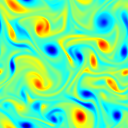
\includegraphics[width=0.4\hsize]{vorticity.eps}
\end{center}
\caption{Vorticity field for the initial random vorticity problem at
$t=18$.}
\label{vorticity}
\end{figure}

Before we carry on, we are going to make two modifications to the
simulation file. First of all, it is not really handy to generate one
file for every image generated. ImageMagick (and most other programs)
can deal with multiple {\sc PPM} images contained within the same
file. Secondly, in the sequence of images we generate, a given value
of the vorticity does not always correspond to the same colour
(because the minimum and maximum values of the vorticity can vary in
time). We can fix that like this:
\begin{verbatim}
1 2 GfsSimulation GfsBox GfsGEdge {} {
  GfsTime { end = 50 }
  GfsRefine 6
  GfsInit {} {
    U = (0.5 - rand()/(double)RAND_MAX)
    V = (0.5 - rand()/(double)RAND_MAX)
  }  
  GfsOutputTime            { istep = 10   } stdout
  GfsOutputProjectionStats { istep = 10   } stdout
  GfsOutputScalarStats     { istep = 10   } stdout { v = Vorticity }
  GfsOutputPPM             { step = 0.1 } vorticity.ppm {
    v = Vorticity 
    min = -10
    max =  10
  }
}
GfsBox {}
1 1 right
1 1 top
\end{verbatim}
We have now specified fixed bounds for the vorticity (using the {\tt
min} and {\tt max} identifiers). Each {\sc PPM} image will be appended to
the same file: {\tt vorticity.ppm}.

How did I choose the minimum and maximum values for the vorticity? The 
line {\tt GfsOutputScalarStats \{ istep = 10 \} stdout \{ v = Vorticity
\}}, writes the minimum, average, standard deviation and maximum
values of the vorticity. By re-running the simulation and looking at
these values it is easy to find a suitable range.

\section{A more complex example with solid boundaries}

In this section we will see how to set up a simulation for the flow past 
a solid body (a half-cylinder) in a narrow channel. While doing that
we will also encounter new ways of displaying simulation results.

\subsection{Domain geometry and boundary conditions}

What we want is a narrow channel ($4\times 1$ for example). From the
previous example, we know that we can build it like this:
\begin{verbatim}
4 3 GfsSimulation GfsBox GfsGEdge {} {
  GfsTime { end = 0 }
}
GfsBox {}
GfsBox {}
GfsBox {}
GfsBox {}
1 2 right
2 3 right
3 4 right
\end{verbatim}
i.e. four boxes, box 1 connected to box 2 horizontally (to the right),
box 2 connected to box 3 horizontally and box 3 connected to box 4
horizontally. Box 1 is centered on the origin and is of size one. All
the other boxes are positioned accordingly. We now have our $4\times
1$ rectangular domain.

\subsubsection{Boundary conditions}

What about boundary conditions? By default Gerris assumes that
boundaries are solid walls with slip conditions for the velocity
(i.e. the tangential stress on the wall is zero). For the moment we
then have defined a rectangular box closed on all sides by solid
walls.

What we really want is to specify an input velocity on the left side
of the box and some sort of output condition on the right side. We can
do that like this:
\begin{verbatim}
4 3 GfsSimulation GfsBox GfsGEdge {} {
  GfsTime { end = 0 }
}
GfsBox { left = GfsBoundaryInflowConstant 1 }
GfsBox {}
GfsBox {}
GfsBox { right = GfsBoundaryOutflow }
1 2 right
2 3 right
3 4 right
\end{verbatim}
The whole left side of the first (leftmost) box is now defined to be a {\tt
GfsBoundaryInflowConstant} object and the whole right side of the last
(rightmost) box a {\tt GfsBoundaryOutflow} object. Again, boundary
conditions objects are all derived from the {\tt GfsBoundary} object
and, as initial conditions, new objects can be easily written by the
user (see also section \ref{morebc}).

We see that {\tt GfsBoundaryInflowConstant} takes one argument which is
the value of the (constant) normal velocity applied to this
boundary. All the other variables (pressure, tracer concentration
etc...) follow a zero gradient condition.

{\tt GfsBoundaryOutflow} implements a simple outflow boundary condition 
where the pressure is set to zero as well as the gradient of all other quantities.

\subsubsection{Solid boundaries}

We now have an empty ``wind tunnel'' with a constant inlet velocity of
norm unity. Gerris can deal with arbitrarily complex solid boundaries
embedded in the quad/octree mesh. The geometry of the solid boundaries
is described using {\sc GTS} triangulated surfaces. In 2D, using 3D
triangulated surfaces seems overkill, as 2D curves would be
enough. However, Gerris being both a 2D and 3D code it deals with 2D
solid boundaries exactly as with 3D ones, even if the simulation is
done only on a 2D cross-section.

Creating 3D polygonal surfaces is not an easy job and is clearly
outside the scope of this tutorial. There are a number of utilities
you can use to do that, including big commercial {\sc CAD}
packages. In general, once you have created a polygonal surface with
one of these tools it should be relatively easy to convert it to the
file format used by {\sc GTS}. In particular, most {\sc CAD} packages
can export to the {\sc STL} (stereolithography) format which is easily
converted to the {\sc GTS} file format using the {\tt stl2gts} utility
which comes with the library.

This tutorial comes (handily) with one such file:
\htmladdnormallinkfoot{{\tt half-cylinder.gts}}
{\gfsweb/half-cylinder.gts}. You can
visualise the surface it describes using a program
called
\htmladdnormallinkfoot{Geomview}{http://www.geomview.org}. To do this,
you first need to convert the {\sc GTS} file to a format Geomview
understands. This can be done using the {\tt gts2oogl} utility like
this:
\begin{verbatim}
% gts2oogl < half-cylinder.gts > half-cylinder.oogl
\end{verbatim}
({\sc OOGL} is the file format used by Geomview). {\tt gts2oogl} has a
number of options. You can have a short explanation of what they do by 
typing:
\begin{verbatim}
% gts2oogl -h
\end{verbatim}
If you now start geomview like this:
\begin{verbatim}
% geomview half-cylinder.oogl
\end{verbatim}
and play around with the pan/rotate/zoom functions of Geomview (read the
manual for details), you should see something like the image on figure 
\ref{half-cylinder}.
\begin{figure}[htbp]
\begin{center}
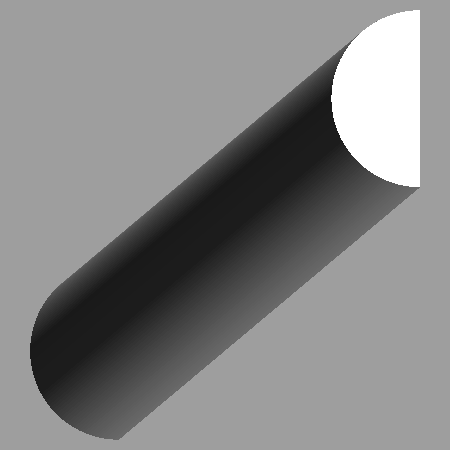
\includegraphics[width=0.3\hsize]{half-cylinder.eps}
\end{center}
\caption{Geomview representation of {\tt half-cylinder.gts}}
\label{half-cylinder}
\end{figure}
You can notice that this is a proper 3D object, even if we are only
going to simulate the flow in a 2D cross-section. It is also important 
that the object is ``tall'' enough so that it spans the entire
``height'' of the 2D domain, as if we were going to simulate the flow
around it in a proper 3D channel with a square cross-section. The
orientation of the surface is also important to define what is inside
(the solid) and what is outside (the fluid).

We can now insert this object in the simulation domain like this:
\begin{verbatim}
4 3 GfsSimulation GfsBox GfsGEdge {} {
  GfsTime { end = 0 }
  GfsSolid half-cylinder.gts
}
GfsBox { left = GfsBoundaryInflowConstant 1 }
GfsBox {}
GfsBox {}
GfsBox { right = GfsBoundaryOutflow }
1 2 right
2 3 right
3 4 right
\end{verbatim}
add what mesh refinement we want and a few things to output:
\begin{verbatim}
4 3 GfsSimulation GfsBox GfsGEdge {} {
  GfsTime { end = 9 }
  GfsRefine 6
  GfsSolid half-cylinder.gts
  GfsInit {} { U = 1 }
  GfsOutputBoundaries {} boundaries
  GfsOutputTime { step = 0.02 } stdout
  GfsOutputProjectionStats { step = 0.02 } stdout
  GfsOutputPPM { step = 0.02 } vorticity.ppm { 
    min = -100 max = 100 v = Vorticity 
  }
  GfsOutputTiming { start = end } stdout
}
GfsBox { left = GfsBoundaryInflowConstant 1 }
GfsBox {}
GfsBox {}
GfsBox { right = GfsBoundaryOutflow }
1 2 right
2 3 right
3 4 right
\end{verbatim}
I have added a new {\tt GfsOutput} object we haven't seen yet: {\tt
GfsOutputTiming}. This object writes a summary of the time taken by
various parts of the solver. You might also have noticed the unusual
{\tt start = end} bit ; this just specifies that this event will only
happen once at the end of the simulation.

Another new output object is {\tt GfsOutputBoundaries}. This object
writes a geometrical summary (in {\sc OOGL}/Geomview format) of the mesh
used, including boundary conditions, solid boundaries and so on.

We also initialise the velocity field on the whole domain
to a constant value (1,0,0). We could have left the
velocity field to its default value of (0,0,0) but, given that we
impose inflow boundary conditions, it would have meant that the
initial velocity would have been strongly divergent. Gerris always
starts a simulation by a projection step (to fix problems like this)
but it is always a good idea to start with the best possible velocity
field.

We can now run the code:
\begin{verbatim}
% gerris2D half-cylinder.gfs
\end{verbatim}
It is going to take a while to complete, but remember that you can
look at files while they are being generated. The first file which
will be generated is {\tt boundaries}. If you load it in Geomview, you
should get something like figure \ref{boundaries} (you probably want
to disable automatic normalization in Geomview by selecting
Inspect$\rightarrow$Appearance$\rightarrow$Normalize$\rightarrow$None).
\begin{figure}[htbp]
\begin{center}
\includegraphics[angle=90,width=0.8\hsize]{boundaries.eps}
\end{center}
\caption{Representation of boundary conditions and solid boundaries}
\label{boundaries}
\end{figure}
The black lines represent the boundaries between solid cells and fluid 
cells. If you zoom in on the half-cylinder, you will see that it is
represented by lines following the grid (it is ``lego-looking''). This 
does not mean that the ``real'' (i.e. computational) solid boundary is 
also lego-looking because fluid cells can be cut by the solid
boundaries, in which case the algorithm properly takes into account
the corresponding cell geometry.

Each {\tt GfsBoundary} object is colour-coded. From the colours in the
picture we see that we have indeed an inflow boundary condition on the
left side (blue) and an outflow boundary condition on the right side
(green).

You can also load in the full half-cylinder geometry we created
before: {\tt half-cylinder.oogl} or visualise the {\sc PPM} files using {\tt 
animate} and {\tt display} as in the previous example. By the way, a
useful feature of {\tt display} is that you can zoom in by clicking on
the middle button in the image being displayed.

\subsection{Saving the whole simulation}

Hmm, this simulation is taking quite a while\dots What if we want to
stop the simulation, make some modifications to the simulation file
and restart where we left from? Or equivalently, save the whole
simulation at regular intervals for latter post-processing?

You can do this using the {\tt GfsOutputSimulation} object. Like this
for example:
\begin{verbatim}
GfsOutputSimulation { step = 0.1 } half-cylinder-%3.1f.gfs {
  variables = U,V,P
}
\end{verbatim}
where {\tt variables} defines which variables you want to save. By
default all the variables are saved.

If you now re-run the simulation, you will get a new file every 0.1
time units. This file is a valid simulation file (like {\tt
half-cylinder.gfs}) and you can use it directly to restart the
simulation from this point onward. If you edit it, you will see that
the general structure is the same as usual but for five pretty big
chunks of data. 

The first chunk starts with {\tt GfsSolid} and is
just the data contained in {\tt half-cylinder.gts} but this time
embedded directly into the simulation file. The goal there is to have
fully self-contained simulations files which you can just move around
without having to keep track of twenty different files.

The four other chunks are each associated with a {\tt GfsBox} and
contain both the topology of the corresponding cell tree but also the
associated physical data, solid boundary definitions etc...

You can of course edit this file, add new outputs and so on and
restart the simulation from where you left it.

\subsection{Visualisation}

\subsubsection{\label{gfsview}GfsView}

GfsView is a tool written specifically to visualise Gerris simulation
files. It is still young but fully usable both for 2D and 3D
simulations. Its main advantage over other options and the reason for
its existence is that it makes full use of the adaptive nature of the
octree representation at the visualisation level. The octree structure
is used within GfsView to dynamically select the appropriate level of
refinement depending on the viewpoint, zoom and rendering speed. It is
also used to efficiently compute complex geometrical entities such as
isosurfaces or cut-planes.

The more classical viewers such as openDX or MayaVi are designed for
either regular Cartesian grids or fully-unstructured meshes and do not
take advantage of the octree representation (worse still, the octree
representation first needs to be converted to Cartesian or
fully-unstructured meshes before being imported into these programs).

To install GfsView, you need to have the
\htmladdnormallinkfoot{Gtk+}{http://www.gtk.org} toolkit installed on
your system. If you are running a Linux machine, Gtk+ is most probably
already installed. You will also need the
\htmladdnormallinkfoot{GtkGlExt}{http://gtkglext.sourceforge.net/}
OpenGL extension to Gtk+.

If you are running a Debian-based system, you can install these packages using
\begin{verbatim}
% apt-get install libgtkglext1-dev
\end{verbatim}

If you then download a recent version of GfsView from the Gerris web
site (either an official release or a snapshot) and do the now classical:
\begin{verbatim}
% gunzip gfsview.tar.gz
% tar xvf gfsview.tar
% cd gfsview
% ./configure --prefix=/home/joe/local
% make
% make install
\end{verbatim}
you will be able to start GfsView using:
\begin{verbatim}
% gfsview2D half-cylinder-0.5.gfs
\end{verbatim}
Note that you can also install the most recent GfsView version using
darcs and {\tt http://gerris.dalembert.upmc.fr/darcs/gfsview-stable} as source
repository (you will also need to install Gerris this way, see section
\ref{build_darcs} for details).

Clicking on ``Linear'', ``Vectors'' and ``Solid'' in the toolbar and
changing the vector length by editing the properties of the
``Vectors'' object (select the object then choose
``Edit$\rightarrow$Properties'') you should be able to get something
looking like figure \ref{fig:gfsview}. You can pan by dragging the right
mouse button, zoom by dragging the middle button and rotate by
dragging the left button.
\begin{figure}[htbp]
\begin{center}
%% \htmlimage{scale=2.0,external,thumbnail=1}
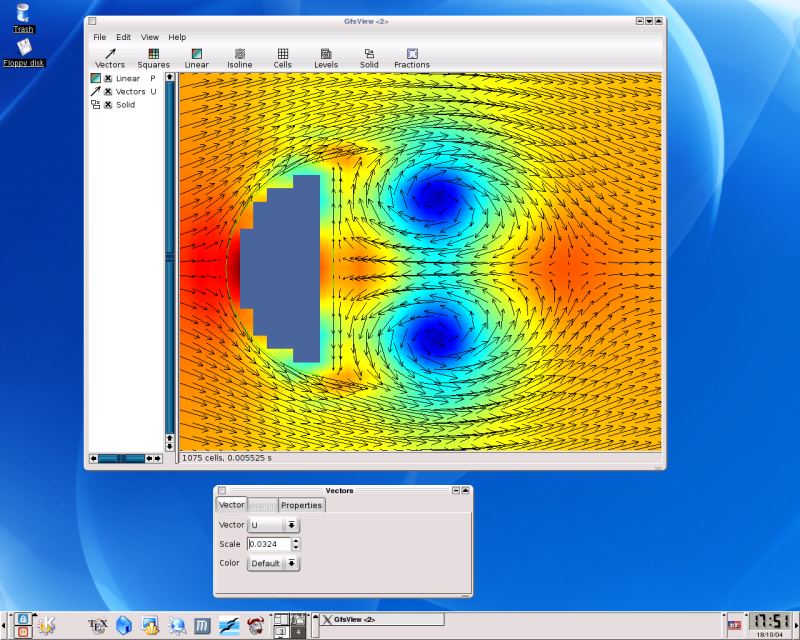
\includegraphics[width=\hsize]{gfsview.eps}
\end{center}
\caption{Screenshot of a GfsView session.}
\label{fig:gfsview}
\end{figure}

While by no means complete, you can already do many things with
GfsView. I hope it is fairly user-friendly so just play with it and
discover for yourself.

\subsubsection{Some post-processing using {\tt gfs2oogl}}

Gerris comes with a utility called {\tt gfs2oogl} which converts
simulation files to various representations in {\sc OOGL} format. We are
just going to look at two types of representations {\tt gfs2oogl} can
do: scalar field cross-sections and vector fields.

First of all, you can access a small summary of the options of {\tt
gfs2oogl} by typing:
\begin{verbatim}
% gfs2oogl2D -h
\end{verbatim}
By default {\tt gfs2oogl} will generate the same output as {\tt
GfsOutputBoundaries} like this:
\begin{verbatim}
% gfs2oogl2D < half-cylinder-0.1.gfs > boundaries.oogl
\end{verbatim}
To generate an {\sc OOGL} representation of a scalar field (a coloured square
for each discretisation cell) do this:
\begin{verbatim}
% gfs2oogl2D -S -z 0 -c Vorticity < half-cylinder-0.5.gfs > squares.oogl
\end{verbatim}
which tells {\tt gfs2oogl} to do a cross-section for $z = 0$ ({\tt -z
0}) represented by squares ({\tt -S}) and colored according to the local
vorticity ({\tt -c Vorticity}).
To generate a vector field representing the velocity try:
\begin{verbatim}
% gfs2oogl2D -V 2 -z 0 < half-cylinder-0.5.gfs > vectors.oogl
\end{verbatim}
where {\tt -V 2} specifies that the maximum length of the vector is
twice the dimension of the smallest cell in the domain.

If you now load all these files in Geomview and do a bit of panning
and zooming around (and possibly tune things like face shading) you
should get an image looking like figure \ref{gfs2oogl}.
\begin{figure}[htbp]
\begin{center}
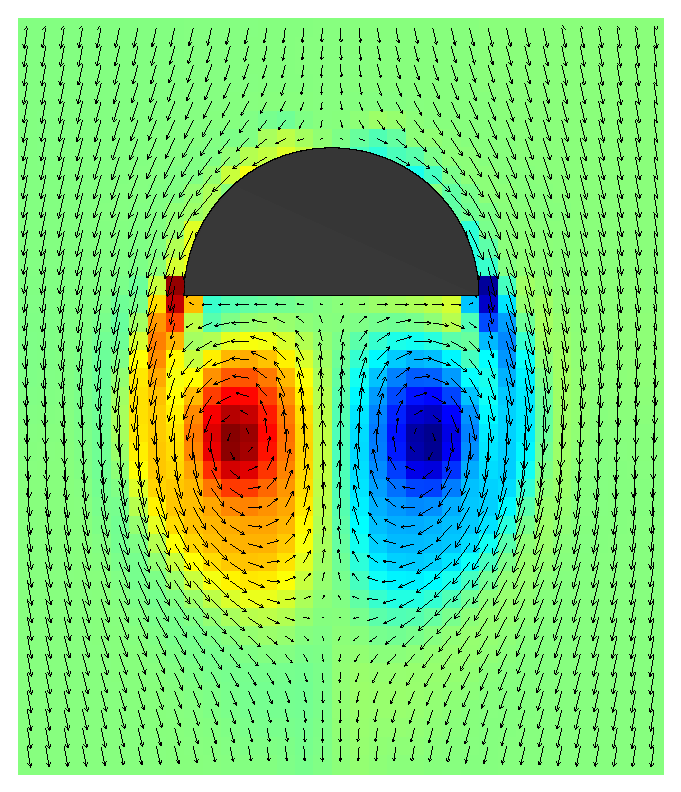
\includegraphics[angle=90,width=0.6\hsize]{gfs2oogl.eps}
\end{center}
\caption{Scalar and vector representation generated using {\tt
gfs2oogl}.}
\label{gfs2oogl}
\end{figure}

\subsection{Using dynamic adaptive mesh refinement}

For the moment our simulation is not very well resolved. We could always 
change the {\tt GfsRefine 6} line to something bigger but it would not
make really good use of the quadtree approach used in Gerris. A code
using a simple regular Cartesian grid approach would be faster and
would produce the same results. Instead we are going to use {\em
dynamic adaptive mesh refinement}, where the quadtree structure of the 
discretisation is used to adaptively follow the small structures of
the flow, thus concentrating the computational effort on the area
where it is most needed. 

This is done using yet another object class: {\tt GfsAdapt}, also derived 
from {\tt GfsEvent}. Various criteria can be used to determine where
refinement is needed. In practice, each criterium will be defined
through a different object derived from {\tt GfsAdapt}. If several {\tt 
GfsAdapt} objects are specified in the same simulation file, refinement 
will occur whenever at least one of the criteria is verified.

For this first example, we will use a simple criterium based on the
local value of the vorticity. A cell will be refined whenever
$$
{|\nabla\times{\bf v}|\Delta x\over\max|{\bf v}|} > \delta,
$$
where $\Delta x$ is the size of the cell and $\delta$ is a
user-defined threshold which can be interpreted as the maximum angular 
deviation (caused by the local vorticity) of a particle traveling at 
speed $\max|{\bf v}|$ across the cell. This criterium is implemented
by the {\tt GfsAdaptVorticity} object.

The general syntax for an {\tt GfsAdapt} object is:
\begin{verbatim}
[GfsEvent] { mincells = 1 maxcells = 100000 minlevel = 1 maxlevel = 10 cmax = 1e-2 }
\end{verbatim}
where {\tt mincells} specifies the minimum number of cells in the
domain, {\tt maxcells} the maximum number of cells, {\tt minlevel} the
level below which it is not possible to coarsen a cell, {\tt maxlevel}
the level above which it is not possible to refine a cell and {\tt
  cmax} the maximum cell cost. The default values are 0 for {\tt
  minlevel} and {\tt mincells} and infinite for {\tt maxlevel} and
{\tt maxcells}. An important point is that, for the moment, it is not
possible to dynamically refine solid boundaries. A simple solution to
this restriction is to always refine the solid boundary with the
maximum resolution at the start of the simulation and to restrict the
refinement using the {\tt maxlevel} identifier in {\tt GfsAdapt}.

What happens if the maximum number of cells is reached? The refinement algorithm will keep the number of cells fixed but will minimize the maximum cost over all the cells. This can be used for example to run a constant-size simulation where the cells are optimally distributed across the simulation domain. This would be done by setting {\tt maxcells} to the desired number and {\tt cmax} to zero.

Following this we can modify our simulation file:
\begin{verbatim}
4 3 GfsSimulation GfsBox GfsGEdge {} {
  GfsTime { end = 9 }
  GfsRefine 7
  GfsSolid half-cylinder.gts
  GfsInit {} { U = 1 }
#  GfsOutputBoundaries {} boundaries
  GfsAdaptVorticity { istep = 1 } { maxlevel = 7 cmax = 1e-2 }
  GfsOutputTime { step = 0.02 } stdout
  GfsOutputBalance { step = 0.02 } stdout
  GfsOutputProjectionStats { step = 0.02 } stdout
  GfsOutputPPM { step = 0.02 } vorticity.ppm {
    min = -100 max = 100 v = Vorticity
  }
  GfsOutputSimulation { step = 0.1 } half-cylinder-%3.1f.gfs {
    variables = U,V,P
  }
  GfsOutputTiming { start = end } stdout
}
GfsBox { left = GfsBoundaryInflowConstant 1 }
GfsBox {}
GfsBox {}
GfsBox { right = GfsBoundaryOutflow }
1 2 right
2 3 right
3 4 right
\end{verbatim}
We have added two lines and commented out (using {\tt \#}) the line
outputting the boundaries (we don't need that anymore, we have the
simulation files).

The first line we added says that we want to refine dynamically the
mesh through the {\tt GfsAdaptVorticity} object applied every timestep
({\tt istep = 1}). The $\delta$ parameter ({\tt cmax}) is set to $10^{-2}$.

The second line we added is a new {\tt GfsOutput} object which displays 
the ``balance'' of the domain sizes across the different processes
(when Gerris is ran in parallel). We will use this to monitor how the
number of cells evolves with time as the simulation refines or
coarsens the mesh according to our vorticity criterium.

We can now run this new simulation. If the previous simulation did not
complete yet, don't be afraid to abort it ({\tt Ctrl-C}), this one is going to
be better (and faster).
\begin{verbatim}
% gerris2D half-cylinder.gfs
\end{verbatim}
If we now look at the balance summary written by {\tt
GfsOutputBalance}, we see that initially ({\tt step: 0}) the total
number of cells (on all levels) is 86966, which corresponds to a
constant resolution of $4\times 2^7\times 2^7=512\times 128$. At step
10 the number of cells is down to 990 with a corresponding increase in 
computational speed. If we now look at the first simulation file we
saved, using:
\begin{verbatim}
% gfs2oogl2D < half-cylinder-0.1.gfs > boundaries
% gfs2oogl2D -S -z 0 -c Vorticity < half-cylinder-0.1.gfs > squares.oogl
\end{verbatim}
we obtain figure \ref{refined1} showing not only the domain boundaries 
as usual, but also the boundaries (thin black lines) between different
levels of refinement.
\begin{figure}[htbp]
\begin{center}
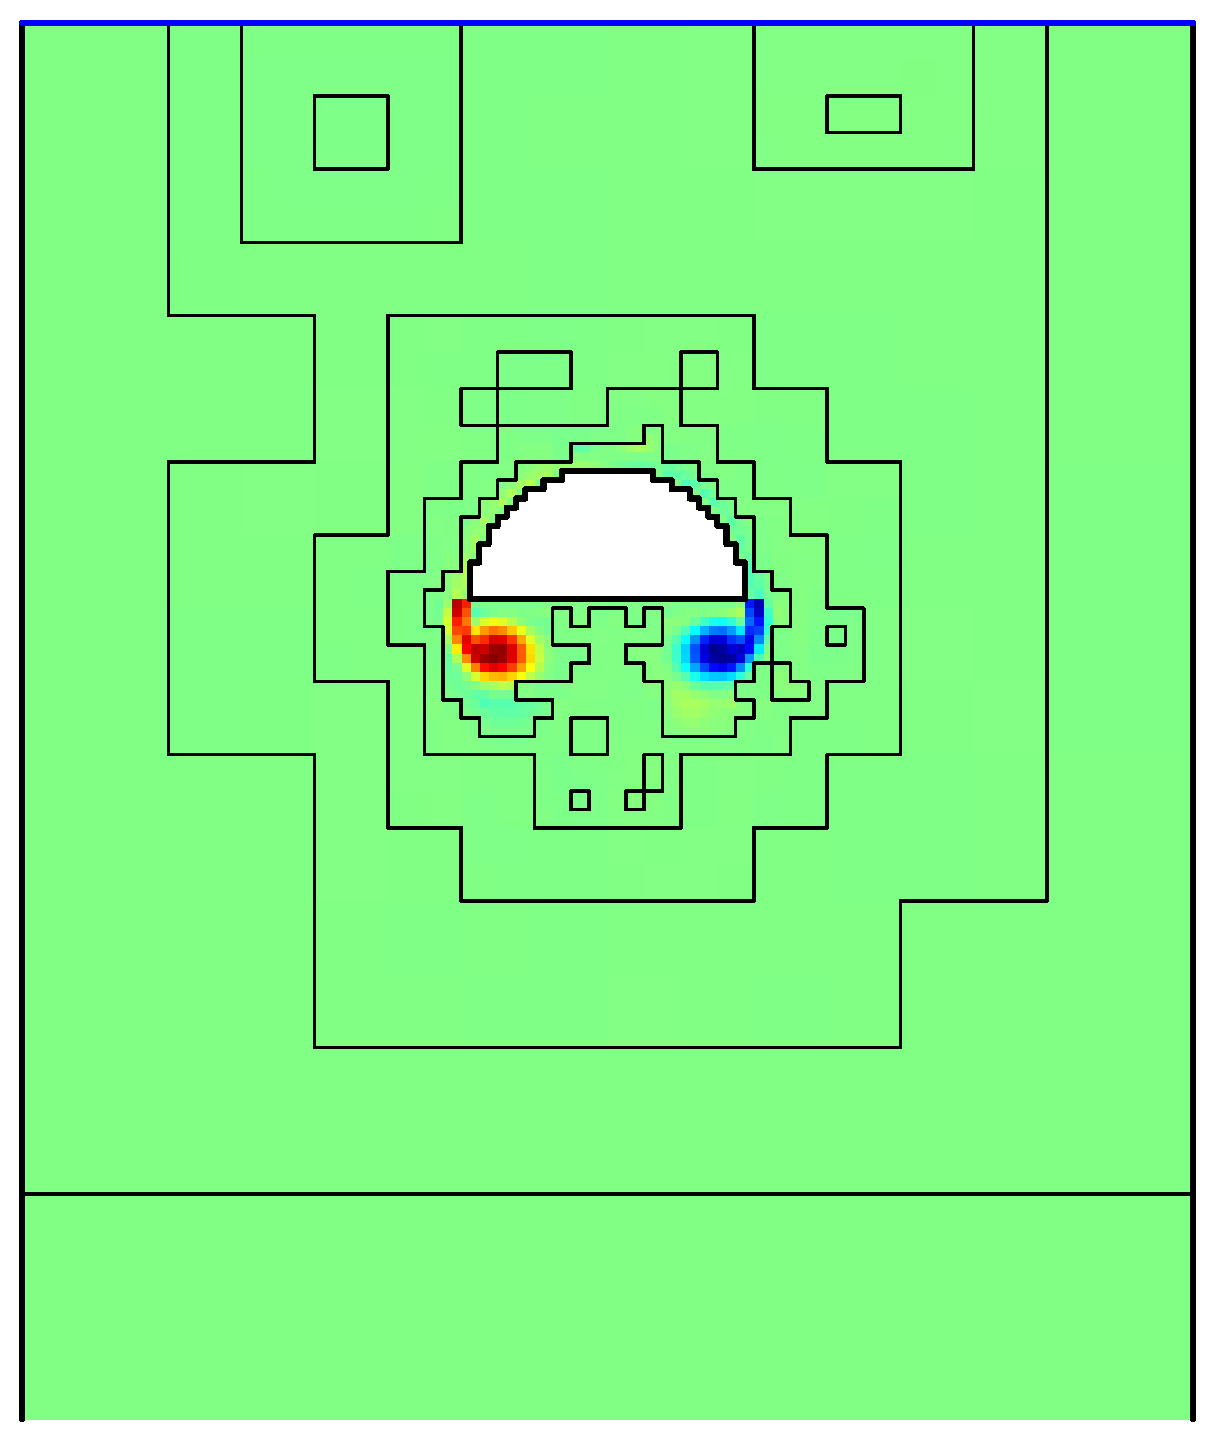
\includegraphics[angle=90,width=0.6\hsize]{refined1.eps}
\end{center}
\caption{Dynamic adaptive mesh refinement $t=0.1$}
\label{refined1}
\end{figure}
We see that the mesh is very refined around the solid and around the
two vortices developing at the trailing edge and very coarse (one cell
per box only) on the downstream part of the domain. If you are not
sure what these thin black lines represent, just switch on the edge
representation in Geomview (using the Inspect$\rightarrow$Appearance menu). You
will get a picture looking like figure \ref{refined1-cells}, showing
all the cells used for the discretisation.
\begin{figure}[htbp]
\begin{center}
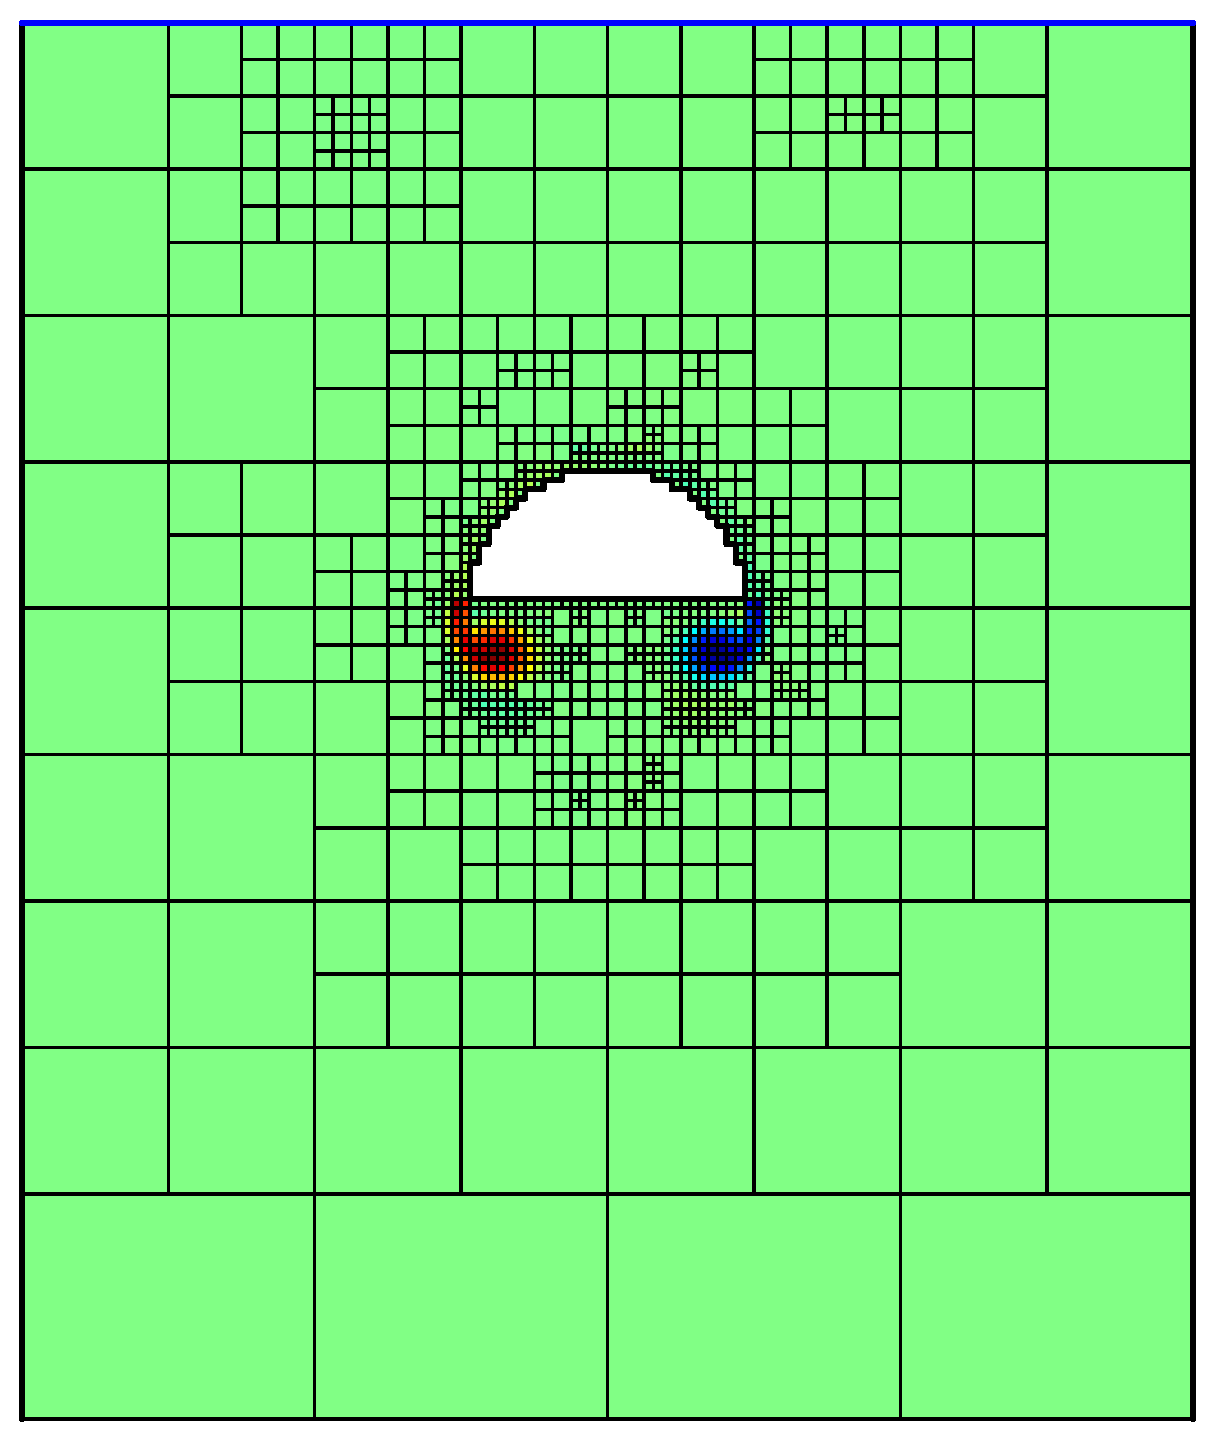
\includegraphics[angle=90,width=0.6\hsize]{refined1_cells.eps}
\end{center}
\caption{Dynamic adaptive mesh refinement $t=0.1$. Detail of the cells.}
\label{refined1-cells}
\end{figure}
As the simulation goes on, you can see the number of cells in the
domain increase as the trailing vortices develop. With a bit of
patience you will get to figure \ref{refined2} showing the fully
developed Von Karman vortex street with patches of increased
resolution following each vortex. Even when the flow is fully
developed using adaptive mesh refinement still saves a factor of \~{}6 in
time and memory use. The advantage of adaptive mesh refinement is even
more obvious in situations where it is necessary to use very large
domains to avoid any contamination of the solution by the boundary
conditions.
\begin{figure}[htbp]
\begin{center}
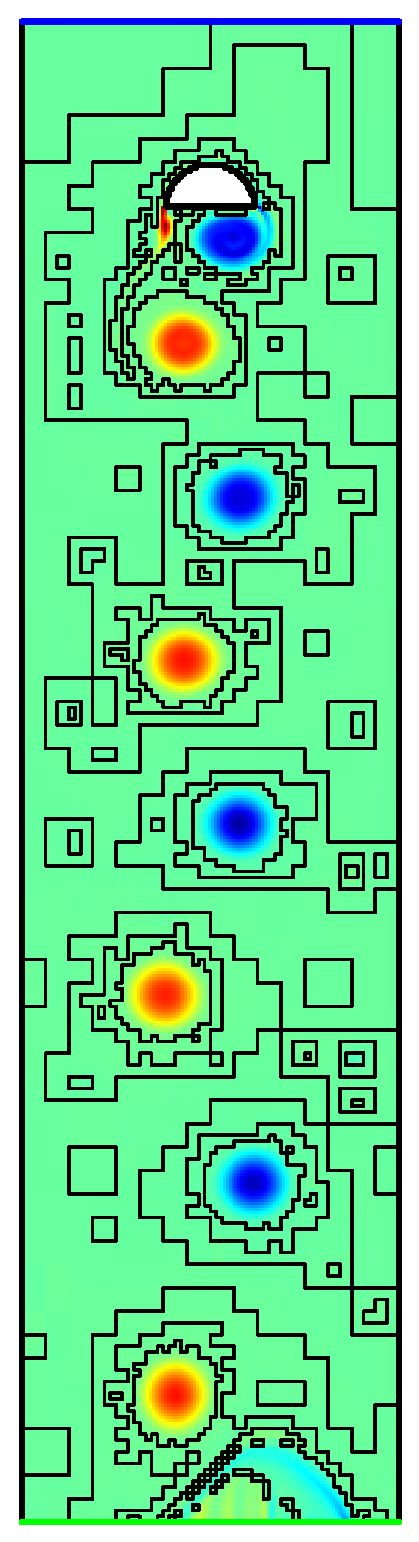
\includegraphics[angle=90,width=0.8\hsize]{refined2.eps}
\end{center}
\caption{Dynamic adaptive mesh refinement $t=9$.}
\label{refined2}
\end{figure}
You should also try to {\tt animate vorticity.ppm} which by now should 
give you a nice animation of the developing trailing vortices becoming 
unstable and generating the Von Karman street. If ImageMagick is
properly installed on your system you can also try:
\begin{verbatim}
% convert vorticity.ppm vorticity.mpg
\end{verbatim}
which will produce a much smaller {\sc MPEG} video file, suitable for
distribution through the network.

\section{Going further}

\subsection{More on boundary conditions}
\label{morebc}

Up to now we have only dealt with ``pre-packaged'' boundary conditions
such as {\tt GfsBoundaryInflowConstant} and {\tt GfsBoundaryOutflow}.
What if you need more specific boundary conditions?

For most practical problems, boundary conditions can be reduced to two
main categories: Dirichlet boundary conditions for which the value of
the variable is set and Neumann boundary conditions for which the
value of the derivative of the variable is set. As we have seen
earlier, the default boundary condition in Gerris is Dirichlet (zero)
for the normal components of the velocity and Neumann (zero) for all
other variables.

Let us say that we want to impose a Poiseuille (parabolic) profile
rather than a constant inflow velocity for the half-cylinder problem
i.e. we want a Dirichlet boundary condition on the normal component of
the velocity ({\tt U}) with an imposed parabolic profile. This can
easily be done in Gerris like this:
\begin{verbatim}
...
GfsBox { left = GfsBoundary {
                  GfsBcDirichlet U { return 1. - 4.*y*y; }
                  GfsBcDirichlet V 0
                }
       }
GfsBox {}
GfsBox {}
GfsBox { right = GfsBoundaryOutflow }
...
\end{verbatim}
Similarly a Neumann boundary condition on variable {\tt X} would use
{\tt GfsBcNeumann X ...}

\subsection{Adding tracers}

In the half cylinder example, it would be nice to be able to visualise
the flow using for example a passive tracer injected at the inlet.
This is very simple, just modify the {\tt half-cylinder.gfs} parameter
file like this:
\begin{verbatim}
4 3 GfsSimulation GfsBox GfsGEdge {} {
  GfsTime { end = 9 }
  GfsRefine 7
  GfsSolid half-cylinder.gts
  GfsVariableTracer {} T
  ...
  GfsOutputPPM { step = 0.02 } tracer.ppm {
    min = 0 max = 1 v = T
  }
  GfsOutputSimulation { step = 0.1 } half-cylinder-%3.1f.gfs {
    variables = U,V,P,T
  }
  ...
}
GfsBox { left = GfsBoundary {
                  GfsBcDirichlet U 1
                  GfsBcDirichlet V 0
                  GfsBcDirichlet T { return y > 0. ? 1. : 0.; }
                } 
       }
...
\end{verbatim}
which will inject tracer {\tt T} at the inlet only in the upper half
of the channel.

The adaptive refinement algorithm shoud also take your tracer into account. Try this
\begin{verbatim}
  ...
  GfsAdaptVorticity { istep = 1 } { maxlevel = 7 cmax = 1e-2 }
  GfsAdaptGradient { istep = 1 } { maxlevel = 7 cmax = 1e-2 } T
  ...
\end{verbatim}
which will adapt using both the gradient of tracer {\tt T} and the vorticity.

You can have any number of tracers you want, they are dynamically
allocated.

\subsection{Adding diffusion terms}

Up to now, we have only considered inviscid, incompressible flows.
Without going into the details, this type of problems require the
solution of two main subproblems: solving a Poisson equation for the
pressure and an advection equation for the momentum and tracers with
the corresponding boundary conditions.

Gerris can also solve a third class of subproblems: diffusion
equations. Diffusion equations are similar to Poisson equations (they
both involve Laplacian operators) and can be solved efficiently using
the same multigrid solver we use for the pressure.

In practice adding diffusion to a given tracer is as simple as adding:
\begin{verbatim}
  ...
  GfsSourceDiffusion {} T 0.01
  ...
\end{verbatim}
to the parameter file, where 0.01 is the value of the diffusion
coefficient.

\subsubsection{\label{diffusionbc}Boundary conditions for diffusion terms}

What if we want to modify the tracer example above so that now the
half-cylinder itself is a (diffusive) source of tracer rather than the
inlet? We need to be able to impose this boundary condition on the
embedded solid surface. On embedded solids, the default boundary
conditions for the diffusion equation is Neumann (zero flux) for
tracers and Dirichlet (no-slip) for the velocity components. To change
that use
\begin{verbatim}
  ...
  GfsVariableTracer T
  GfsSourceDiffusion {} T 0.001
  GfsSurfaceBc T Dirichlet 1
  ...
\end{verbatim}
and change the inlet boundary condition back to
\begin{verbatim}
  ...
  GfsBox { left = GfsBoundary {
                  GfsBcDirichlet U 1
                  GfsBcDirichlet V 0
                } 
       }
  ...
\end{verbatim}

\subsection{Outputs}

\subsection{Boundary conditions}

\section{Running Gerris in parallel}

\section{Learning more}

While this tutorial should give you a good overview of Gerris, it is
by no means a complete description. To learn more you should first
consult the \htmladdnormallinkfoot{Gerris Frequently Asked Questions}{\gfsweb/wiki/index.php/FAQ} and the
\htmladdnormallinkfoot{Gerris object hierarchy}{\gfsweb/wiki/index.php/Object\_hierarchy} which describes each
object and the corresponding file parameters in more detail.

You should also have a look at the \htmladdnormallinkfoot{Gerris
  Examples}{\gfsweb/examples/examples} page for examples of how to
use Gerris for a range of problems. The parameter files are
cross-linked with the reference manual.

Another source of more advanced examples is the \htmladdnormallinkfoot{Gerris test suite}{\gfsweb/tests/tests/index.html}.

If things are still unclear you can ask for help on the
\htmladdnormallinkfoot{{\tt gfs-users} mailing
  list}{\gfsweb/mailinglists.html}. Please note that you
first need to subscribe to the list to be able to post messages.

\section{Do you want to help?}

The idea behind Gerris and other free software projects is that
transparency, free exchange of information and cooperation benefit
individuals but also society as a whole. If you are a scientist, you
know that these same principles are also keys to the efficiency of
Science.

Helping with Gerris development can be done in various ways and aside
from giving you this altruistic, warm fuzzy feeling of helping others
will also benefit you directly. A few concrete simple ways of helping
are (in approximate order of difficulty):
\begin{itemize}
\item Use the code, comment on the problems you find, what you like, don't like about it.
\item Share your results with other Gerris users, write a web page
  about the problem you solved using Gerris etc\dots
\item If you publish papers using Gerris, send me the reference. It is
  very useful to be able to show evidence of wider usage when seeking
  continued funding for the project.
\item Also, if Gerris capabilities are central to your article feel
  free to ask me to be a co-author on your paper\dots
\item Have a look at the Gerris internals (write your own modules) and share them with us.
\item Think of ways to extend Gerris for your own problems, implement
  them and share them with us (you can count on my and other
  developers' help).
\end{itemize}

\end{document}
